\section{Introduction}
%----------------------

{\setbeamercolor{background canvas}{bg=LemonChiffon}
\begin{frame}
\frametitle{}
{\fontsize{50}{60}\selectfont Introduction:}
{\huge What? Why? How?} 

\end{frame}
}

%--------------------------------------------------------------------------------------------------------------
\begin{frame}
\frametitle{What is Python?}

Programming language:
\begin{enumerate}
\item interpreted \comment{instructions executed directly}
\item dynamically typed \comment{type checking at run-time}
\item object-oriented \comment{classes, objects, methods, \ldots}
\item high-level \comment{strong abstraction}
%\item simple, easy to learn syntax
\end{enumerate}

\vfill


\includegraphics[height=1.5cm]{logo_python}


\url{https://www.python.org}

\end{frame}

% 1st example here with strings


%--------------------------------------------------------------------------------------------------------------
\begin{frame}[c]
\frametitle{Why Python?}

\onslide*<1>{
\begin{enumerate}
\item Simple, easy to learn syntax
\item Open
\item Large user community \comment{doc, support, packages}
\end{enumerate}
}

\onslide*<2>{
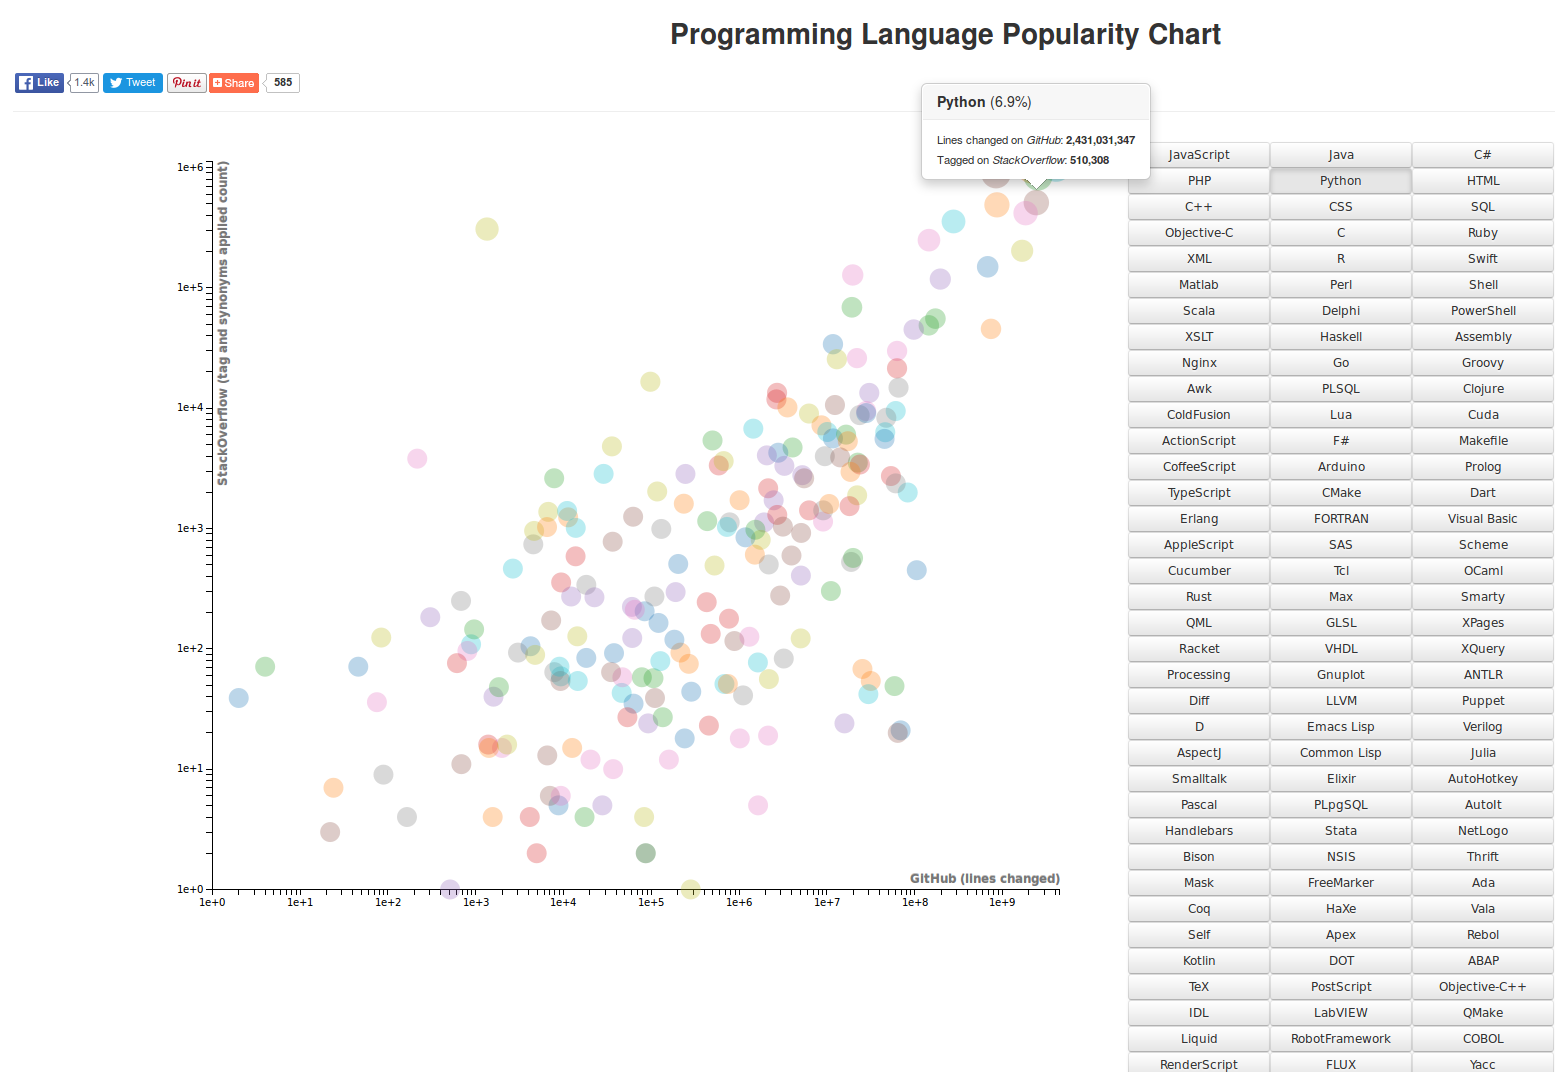
\includegraphics[width=.9\textwidth]{langpop_corger_nl}\\
{\scriptsize Source: \url{http://langpop.corger.nl/}}
}
\end{frame}


%--------------------------------------------------------------------------------------------------------------
\subsection{Python vs. Matlab}

\begin{frame}[fragile]
\frametitle{Python vs. Matlab}
\footnotesize

\begin{table}
\scriptsize
\begin{tabular}{p{.4\textwidth}p{.4\textwidth}}
\toprule
Python  	  				& Matlab\\
\midrule
\textbf{General}			& \\
programming language		& programming language + numerical computing environment\\
open						& proprietary algorithms\\
general purpose				& linear algebra\\
\midrule
\textbf{Indexing} 			& 	\\
a[0]						& a(1) \\
a[-1]						& a(end)\\
a[::2]						& a(1:2:end)\\
\midrule
\textbf{Functions}			& \\
a.max()						& max(a)\\
a.shape()					& size(a)\\
\bottomrule
\end{tabular}
\end{table}

\vfill

Numpy for Matlab users:\\
\url{https://docs.scipy.org/doc/numpy-dev/user/numpy-for-matlab-users.html}

\end{frame}


%--------------------------------------------------------------------------------------------------------------
\begin{frame}[t, fragile]
\frametitle{Quick example: hello.py}

{\huge
\faLaptop
}


\begin{onlyenv}<2>
\begin{lstlisting}[language=python]
#!/usr/bin/python
# -*- coding: utf-8 -*-
'''
This function prints "Hello world"
'''

def hello():
  print "Hello world"
  return

def main():
  hello()

if __name__ == '__main__':
  main()
\end{lstlisting}
\end{onlyenv}

{\normalsize
\begin{enumerate}
\item<3-> Try to document you code
\item<4-> Use 
\begin{lstlisting}[language=python]
# -*- coding: utf-8 -*- 
\end{lstlisting}
if you're using non-ascii characters
\item<5-> In Python~3: 
\begin{lstlisting}[language=python]
print("Hello world!")
\end{lstlisting}
\item<6-> Indentation matters!
\end{enumerate}
}
\end{frame}

%--------------------------------------------------------------------------------------------------------------
\subsection{Definitions and data types}
\begin{frame}[fragile]
\frametitle{A few definitions}

\begin{description}
\item[Object:] Python's abstraction for data\\
\url{https://docs.python.org/2/reference/datamodel.html#index-0}
\item[Function:] series of statements which returns some value to a caller\\
\url{https://docs.python.org/2/glossary.html#term-function}
\item[Module:] file containing Python definitions and statements\\
\url{https://docs.python.org/2/tutorial/modules.html}
\item[Class:] logical grouping of data and methods (functions)\\
\url{https://docs.python.org/2/tutorial/classes.html}
\end{description}

\end{frame}

%--------------------------------------------------------------------------------------------------------------

\begin{frame}[t, fragile]
\frametitle{Data types}

\begin{enumerate}
\item<1-> Numbers
\item<2-> String
\item<3-> List
\item<4-> Tuple
\item<5-> Dictionary
\end{enumerate}

\onslide<1-5>{\textbf{Example:}}

\begin{onlyenv}<1>
\begin{lstlisting}[language=python]
g = 9.81
h = 4.135667662e-15
\end{lstlisting}
\end{onlyenv}

\begin{onlyenv}<2>
\begin{lstlisting}[language=python]
name = "Rickman"
s = "this is a string"
\end{lstlisting}
\end{onlyenv}

\begin{onlyenv}<3>
\begin{lstlisting}[language=python]
list = ['one', 2, 'three', 'four', 5]
\end{lstlisting}
\end{onlyenv}


\begin{onlyenv}<4>
\begin{lstlisting}[language=python]
tuple1 = ('one', 2, 'three', 'four', 5)
tuple2 = (1, '1', 'one', [1, 2], (1, 2, 3))
\end{lstlisting}

Tuples are \textit{immutable} \comment{(fixed value)}
\end{onlyenv}


\begin{onlyenv}<5>
\begin{lstlisting}[language=python]
email = {'Evan': 'emason@imedea.uib-csic.es',\
         'Irene': 'irene.laiz@uca.es',\
         'Charles': 'ctroupin@socib.es'}
email['Irene']
'irene.laiz@uca.es'
\end{lstlisting}
\end{onlyenv}

\begin{onlyenv}<6>
More details:\\
\url{https://docs.python.org/2/tutorial/datastructures.html#}

\vspace{1cm}

{\huge \faLaptop}

\end{onlyenv}

\end{frame}

%--------------------------------------------------------------------------------------------------------------
\subsection{Resources, tutorials, books}
\begin{frame}
\frametitle{Resources}

\onslide*<1>{
Web:
\begin{itemize}
\item \url{https://docs.python.org/2.7/tutorial/index.html}
\item \url{https://developers.google.com/edu/python/introduction?hl=en} \comment{tutorial + exercises}
\item \url{http://www.python-course.eu}
\item \url{http://www.learnpython.org} \comment{online code execution}\\
\url{https://pythonprogramming.net}
\item \url{https://www.gitbook.com/book/djangogirls/djangogirls-tutorial} 
\end{itemize}
}

\onslide*<2>{
Learning platforms:
\begin{itemize}
\item \href{https://www.udacity.com/course/programming-foundations-with-python--ud036}{
Programming Foundations with Python
Learn Object-Oriented Programming} \comment{(7 weeks)}
\item \href{https://www.codecademy.com/learn/python}{Code Academy} \comment{(13 hours)}
\end{itemize}
}

\onslide*<3>{
Youtube:
\begin{itemize}
\item \href{https://www.youtube.com/watch?v=cpPG0bKHYKc}{Python Beginner Tutorial (For Absolute Beginners)}\comment{(4 parts)}
\item \href{https://www.youtube.com/watch?v=tKTZoB2Vjuk}{Google Python Class} \comment{(7 $\times$ 30 minutes)}
\item \href{https://www.youtube.com/watch?v=9uq3w6JJS00}{Zero to Hero with Python} \comment{(11 hours)}
\end{itemize}
}

\onslide*<4>{
Books:
\begin{itemize}
\item \textit{Learn Python the hard way}, Z.A.~Shaw, 2013\\
\url{http://learnpythonthehardway.org/book/}
\item \textit{Learning Python, 5th Edition}, M.~Lutz, 2013
\item \textit{Python Programming: An Introduction to Computer Science}, J.M. Zelle, 2002 
\end{itemize}

\vspace{1cm}

Complete list: \url{https://wiki.python.org/moin/PythonBooks}
}

\end{frame}

%--------------------------------------------------------------------------------------------------------------
\begin{frame}[fragile]
\frametitle{Python 2 vs Python 3}

Some differences:
\begin{itemize}
\item Print function
\item Integer division
\item Unicode
\item \ldots
\end{itemize}

Python 3.x = present and future of the language

\vfill

More details:\\
\href{https://wiki.python.org/moin/Python2orPython3}{Python 2 or Python 3}\\
\href{https://jakevdp.github.io/blog/2013/01/03/will-scientists-ever-move-to-python-3/}{Will Scientists Ever Move to Python 3?}

\end{frame}


%--------------------------------------------------------------------------------------------------------------

\begin{frame}[fragile]
\frametitle{Objectives of the course}

\begin{enumerate}
\item<1-> Use Python to solve oceanography-related problems
\item<2-> Read/write various types of files
\item<3-> Generate high-quality figures
\item<4-> Find resources on the internet for specific problems
\end{enumerate}

\vspace{.5cm}

\onslide<5->{\textbf{What we won't (can't) do:}\\
teach you how to be a good programmer}

\end{frame}

%--------------------------------------------------------------------------------------------------------------

\begin{frame}
\frametitle{About the trainers}


% maybe add pictures
\onslide<1->{\textbf{Evan Mason}\\
Oceanographer\\
Post-doctoral researcher at \href{http://imedea.uib-csic.es/}{IMEDEA}\\
10-year experience with Python

}

\vspace{1cm}

\onslide<2->{\textbf{Charles Troupin}\\
Engineer, oceanographer\\
Head of \href{http://socib.es/}{SOCIB} Data Center\\
2.5-year experience with Python
}



\end{frame}

%--------------------------------------------------------------------------------------------------------------

\begin{frame}[t]
\frametitle{Structure of the course}

\begin{enumerate}
\item<1-> Reading/writing
\item<2-> Time series 
\item<3-> 2-D fields
\item<4-> Functions, classes, modules
\end{enumerate}

\vspace{1cm}

\includegraphics<1->[height=1.5cm]{python_idle2}~\includegraphics<2->[height=1.5cm]{IR_TS_MO_61198_monthly}~\includegraphics<3->[height=1.5cm]{anomalies_10profiler-glider_201507}~\includegraphics<4->[height=1.5cm]{eddy_tracking_ex}


\end{frame}

